%!TEX root = restart.tex
\section{Numerical results for model predictive control implementations\label{sec:Numerical-results-for}}

To demonstrate the effectiveness of using the adjoint ramp metering
method to compute gradients, we implemented the algorithm on practical scenarios with field experimental data.
The algorithm can then be used as a gradient computation subroutine
inside any descent-method optimization solver that takes advantage
of first-order gradient information. Our implementation makes use
of the open-source \emph{IpOpt} solver~\cite{Andreas2005}, an interior point, nonlinear program optimizer. To serve
as comparisons, two other case scenarios were run:
\begin{enumerate}
	\item No control: the metering rate is set to 1 on all onramps at all times.
	\item Alinea~\cite{Papageorgiou1991}: a well-adopted, feedback-based ramp metering
	algorithm commonly used in the practicioner's community. Alinea is computationally efficient and decentralized,
	making it a popular choice for large networks, but does not take estimated
	boundary flow data as input. Since Alinea has a number of tuning parameters,
	we perform a \emph{modified} grid-search technique over the different
	parameters that scales linearly with the number of onramps, and select
	the best-performing parameters, in order to be fair to this framework. A \emph{full} grid-search approach
	scales exponentially with the number of onramps, rendering it infeasible
	for moderate-size freeway networks.
\end{enumerate}
\textbf{Note: } To demonstrate the reduced computation time associated with the adjoint approach, we also implemented gradient descent using a finite differences approach to compute the gradient, similar to~\cite{Frejo2011,Ramon2013}, but it proved to be computationally infeasible for even small, synthetic
networks. Running ramp metering on even a network of 4 links over
6 time-steps for 5 gradient steps took well over 4 minutes,
rendering the method useless for real-time applications. The comparison
of running times of finite differences versus the adjoint method is given in
Figure~\ref{fig:Running-time-of}. We do not consider the finite differences in further results, due to the impractically large running times, which only becomes worse as the problem scales to larger networks and time horizons.
\begin{figure}
	\begin{centering}
		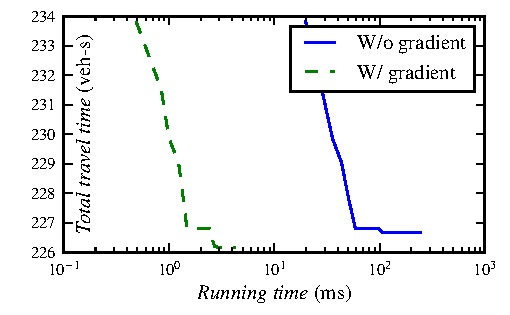
\includegraphics[width=0.5\columnwidth]{images/itergrad}
		\par\end{centering}
				
		\caption{Running time of metering algorithm with and without gradient computations.
			Network consists of 4 links and 6 time-steps with synthetic boundary
			flux data. The method using gradient computations via the adjoint
			method converged well before the first step was completed with the
			method that used perturbations to compute the gradient.\label{fig:Running-time-of}}
		\end{figure}
				
				
				
		\subsection{Implementation on I15S in San Diego\label{sub:Network}}
				
		As input into the optimization problem, we constructed a model of
		a 19.4 miles
 stretch of the I15 South freeway in San Diego,
		California between San Marcos and Mira Mesa.The network has $\nlinks=$
		125
 links, $\ncontrols=$9
 onramps,
		with boundary data specified for $\ntime=$ 1800 time-steps,
		for a time horizon of 120.0 minutes
 given $\Delta t=$ 4 seconds
.
		The network is shown in Figure~\ref{fig:Model-of-section}.
		\begin{figure}
			\begin{centering}
				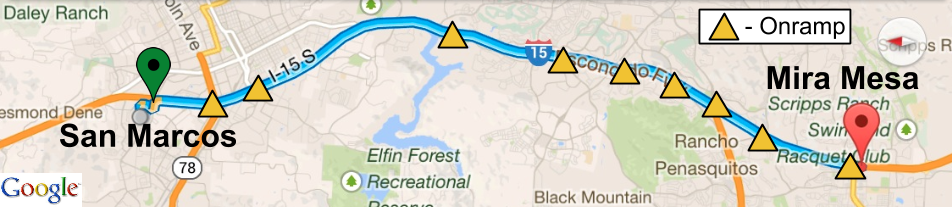
\includegraphics[width=0.7\columnwidth]{images/map}
				\par\end{centering}
								
				\caption{Model of section of I15 South in San Diego, California. The freeway
					section spanning~19.4 miles was split into~125 links with 9 onramps.\label{fig:Model-of-section}}
				\end{figure}
								
								
				Link length data was obtained using the Scenario Editor software developed
				as part of the \textit{Connected Corridors} project, a collaboration between
				UC Berkeley and PATH research institute in Berkeley, California.
				Fundamental diagram parameters, split ratios, and boundary data were
				also obtained using calibration techniques developed by Connected
				Corridors. Densities resulting in free-flow speeds were chosen as
				initial conditions on the mainline and onramps. The data used in calibration
				was taken from PeMS sensor data~\cite{Chen2003} during a morning rush hour period,
				scaled to generate congested conditions. The input data was chosen
				to demonstrate the effectiveness of the adjoint ramp metering method
				in a real-world setting. A profile of the mainline and onramps during
				a forward-simulation of the network is shown in Figure~\ref{fig:Density-and-queue}
				under the described boundary conditions.
				\begin{figure}[b]
					\subfloat[Density profile. The units are the ratio of a link's vehicle density
						to a link's jam density.\label{fig:Density-profile.}]{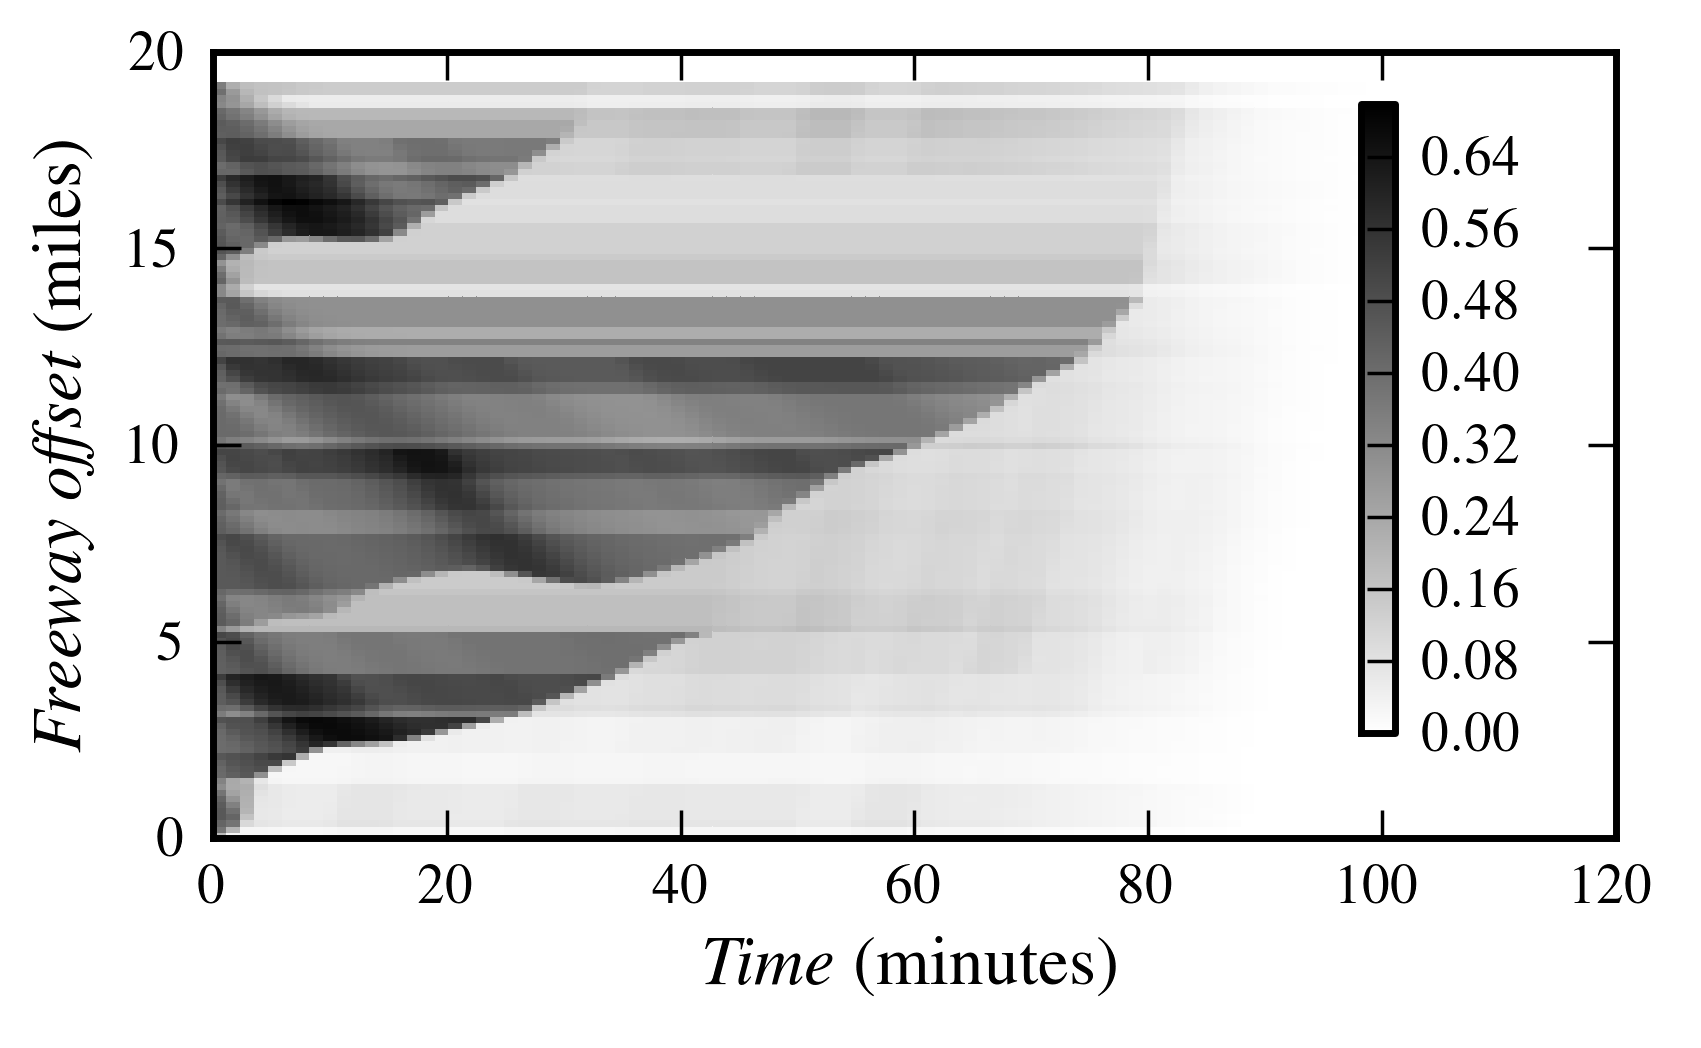
\includegraphics[width=0.45\columnwidth]{images/ncdensity}
																
								}\hfill{}\subfloat[Onramp queue profile in units of vehicles.\label{fig:Density-profile.-2}]{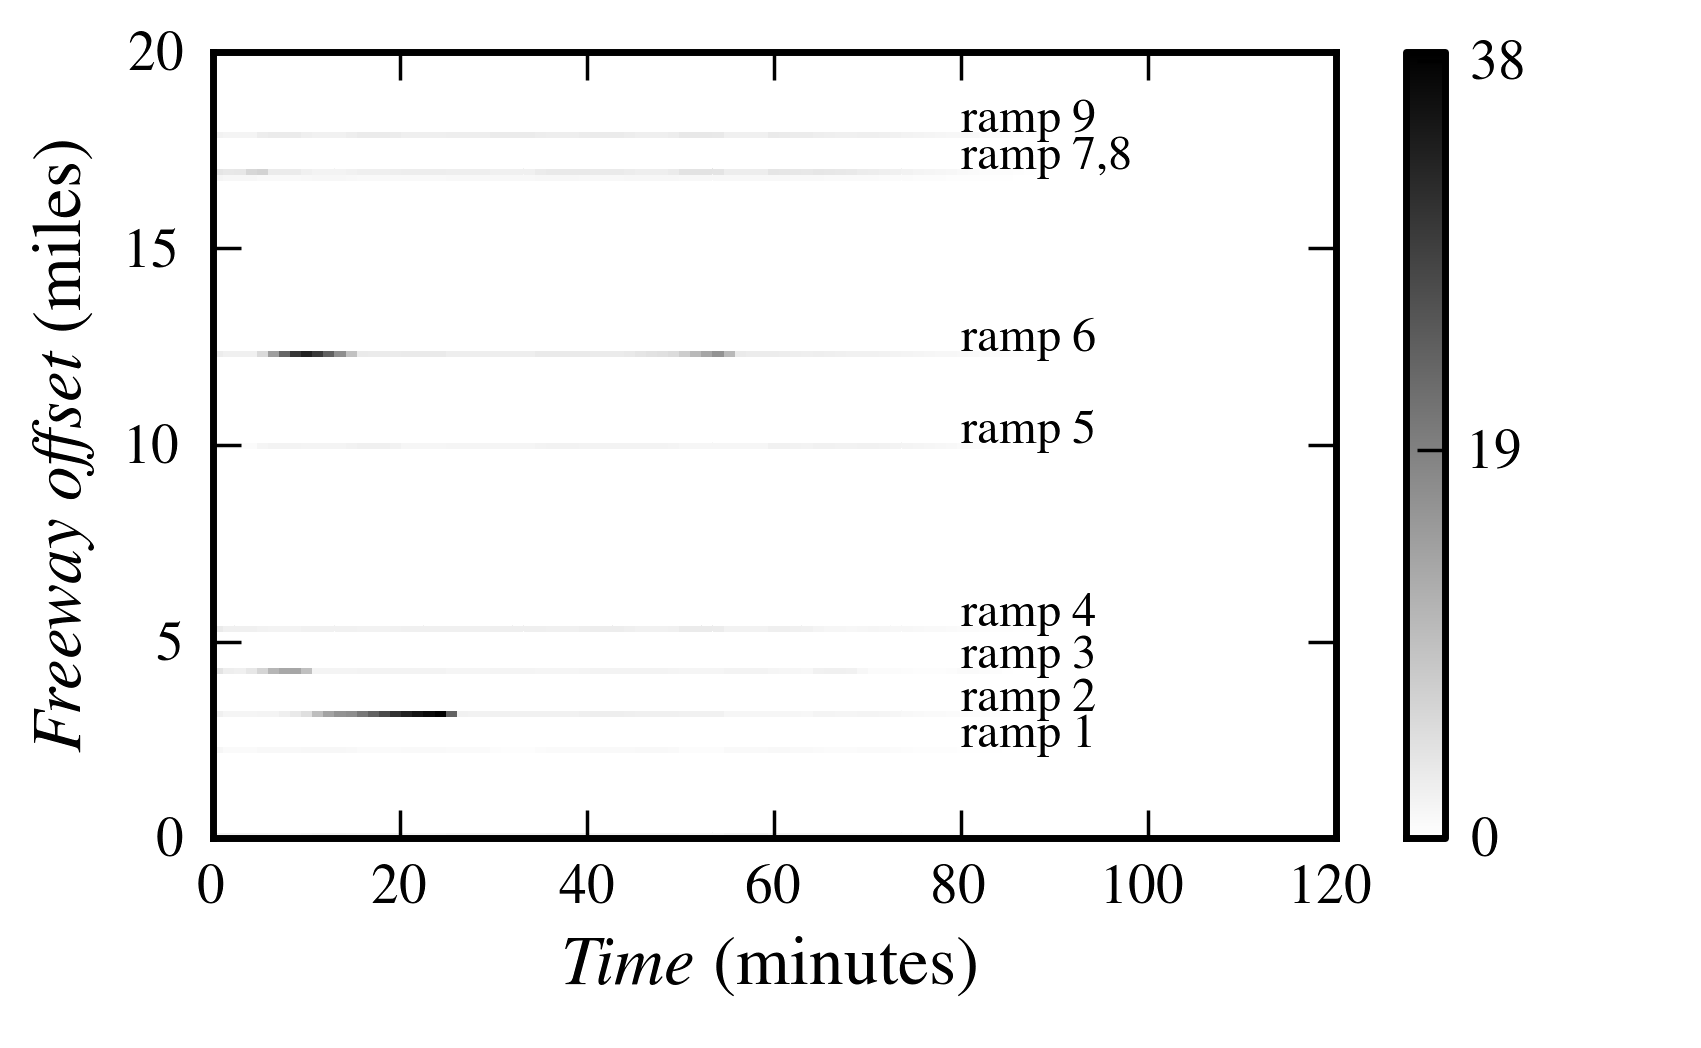
\includegraphics[width=0.45\columnwidth]{images/ncqueue}
																		
								}
																
								\caption{Density and queue profile of no-control freeway simulation. In the
									first 80 minutes, congestion pockets form on the freeway and queues
									form on the onramps, then eventually clear out before 120 minutes.\label{fig:Density-and-queue}}
							\end{figure}
														
														
														
							\subsection{Finite-horizon optimal control\label{sub:Finite-horizon-optimal-control}}
														
														
							\paragraph{Experimental setup.}
														
							The adjoint ramp metering algorithm is compared to the reactive Alinea
							scheme, for which we assume that perfect boundary conditions and initial conditions
							are available. The metric we use to compare the different strategies is \emph{reduced-congestion} percentage, $\bar{c} \in \left(-\infty,100\right]$, which we define as:
							\[
							\bar{c} = 100 \left(1 - \frac{c_c}{c_{nc}}\right)
							\], where $c_c, c_{nc} \in \mathbb{R}_+$ are the \emph{congestion} resulting from the \emph{control} and \emph{no-control} scenarios, respectively. We use the metric for congestion as defined in~\cite{Skabardonis2003}; for a given section of road $s$ and time period $t$, the congestion is given as
							\[
							c\left(s,t\right) = \sum_{\left(\sigma\in s, \tau\in t\right)} \max \left[\text{TTT}\left(\sigma,\tau\right) - \frac{\text{VMT}\left(\sigma, \tau\right)}{V_r}, 0\right]
							\], where $\text{VMT}$ is total vehicle miles traveled, and $\text{TTT}$ is total travel time over the link $\sigma$ and time-step $\tau$. Since it is infeasible to compute the global optimum for all cases, a reduced congestion of 100\% serves as an upper bound on the possible amount of improvement.

							\paragraph{Results.}
														
							\begin{figure}[t]
								\subfloat[Density difference profile in units of \emph{change in density} from the control scenario to the no control scenario over the jam density of the link.\label{fig:long-sim-density}]{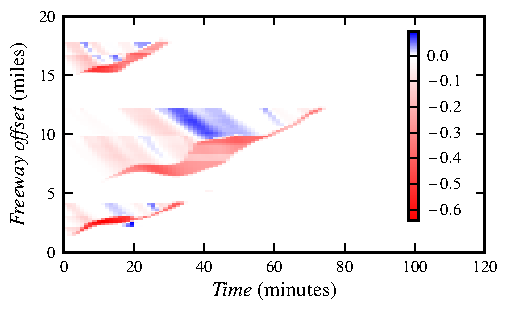
\includegraphics[width=0.45\columnwidth]{images/densdiff}
																		
									}\hfill{}\subfloat[Queue difference profile in units of vehicles.\label{fig:long-sim-queue}]{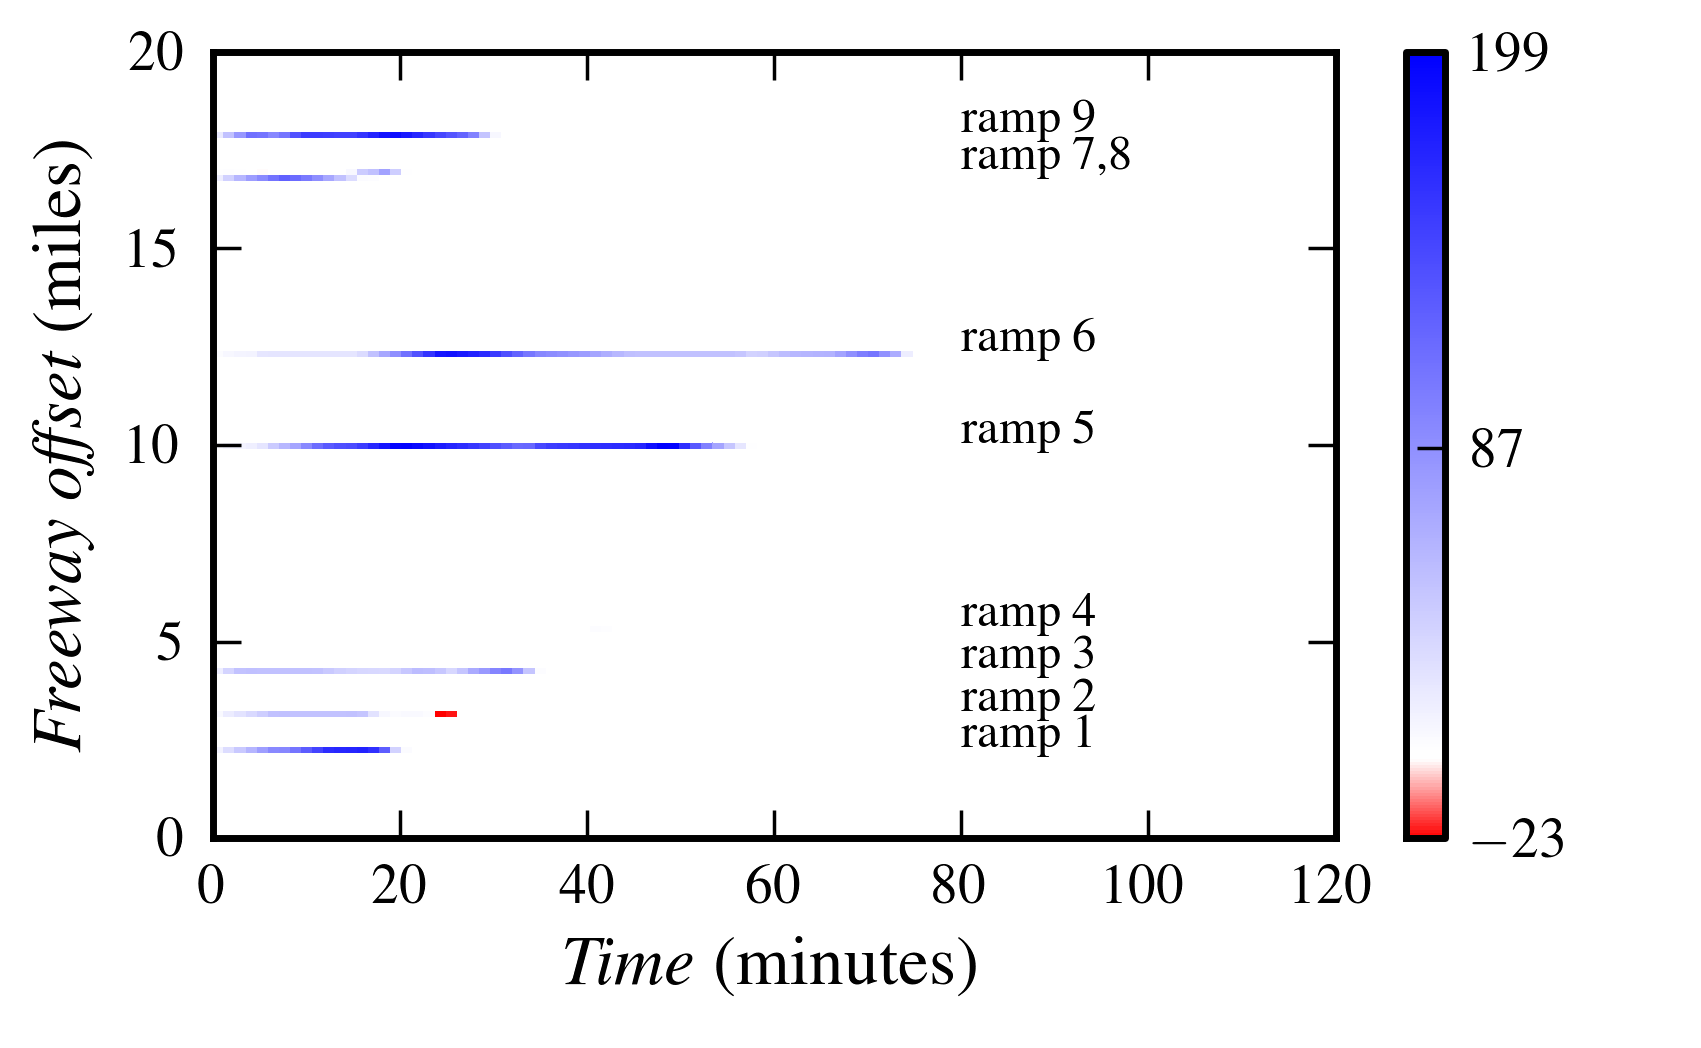
\includegraphics[width=0.45\columnwidth]{images/queuediff}
																		
								}
																
								\caption{Profile differences for mainline densities and onramp queues. Evidenced
									by the mainly negative differences in the mainline densities and the
									mainly positive differences in the onramp queue lengths, the adjoint
									ramp metering algorithm effectively limits onramp flows in order to
									reduce mainly congestion.\label{fig:long-sim}}
							\end{figure}
														
														
							Figure~\ref{fig:long-sim} shows a difference profile for both density and queue lengths between the
							no control simulation and the simulation applying the ramp metering
							policy generated from the adjoint method. Negative differences in
							Figures~\ref{fig:long-sim-density} and~\ref{fig:long-sim-queue}
							indicate where the adjoint method resulted in fewer vehicles for the
							specific link and time-step. The adjoint method was successful in
							appropriately deciding which ramps should be metered in order to improve
							throughput for the mainline.
							\begin{figure}
								\begin{centering}
									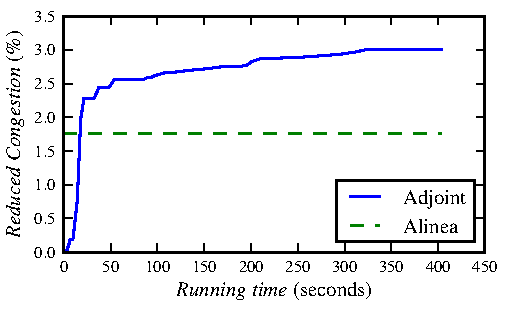
\includegraphics[width=0.65\columnwidth]{images/longsim}
									\par\end{centering}
									\caption{Reduced congestion versus simulation time for freeway network. The results
										indicate that the algorithm can run with performance better than Alinea
										if given an update time around 15 minutes.}\label{fig:running-time}
								\end{figure}
																
																
								Running time analysis shows that the adjoint method can produce beneficial
								results in real-time applications. Figure~\ref{fig:running-time} details the improvement of the adjoint method as a function of the overall running time of the algorithm. After just a few gradient steps, the
								adjoint method outperforms the Alinea method. Given that the time
								horizon of two hours is longer than the period of time one can expect
								reasonably accurate boundary flow estimates, more practical simulations
								with shorter time horizons should permit more gradient steps in a
								real-time setting.
																
								While the adjoint method leads to queues with a considerable number of cars in some onramps, this can be addressed by introducing barrier terms into the cost function that limit the
								maximum queue length. The Alinea method tested for the I15 network
								had no prescribed maximum queue lengths as well, but was not able
								to produce significant improvements in total travel time reduction, while the adjoint method was
								more successful.
																
																
								\subsection{Model predictive control\label{sub:Model-predictive-control}}
																
								To study the performance of the algorithm under noisy input data,
								we embed both our adjoint ramp metering algorithm and the Alinea algorithm
								inside of a \emph{Model predictive control }(MPC) loop.
																
																
								\paragraph{Experimental setup.}
																
								The MPC loop begins at a time $t$ by estimating the initial conditions
								of the traffic on the freeway network and the predicted boundary fluxes
								over a certain time horizon $T_{h}$. These values are noisy, as exact
								estimation of these parameters is not possible on real freeway networks.
								The estimated conditions are then passed to the ramp metering algorithm
								to compute an optimal control policy over the $T_{h}$ time period.
								The system is then forward-simulated over an update period of $T_{u}\le T_{h}$,
								using the exact initial conditions and boundary conditions, as opposed
								to the noisy data used to compute control parameters. The state of
								the system and boundary conditions at $t+T_{u}$ are then estimated
								(with noise) and the process is repeated.
																
								A non-negative\emph{ noise factor}, $\noiseFactor \in \R_+$, is used to study how the adjoint
								method and Alinea perform as the quality of estimated data decreases. If $\discrete{}{}$ is the actual density for a cell and timestep, then the density $\bar{\discrete{}{}}$ passed to the control schemes is given by:
								\[
									\bar{\discrete{}{}}=\discrete{}{}*(1+\noiseFactor*R)
								\]
								where $R$ is a uniformly distributed random variable with mean $0$
								and domain $\left[-0.5,0.5\right]$. The noise factor was applied
								to both initial and boundary conditions.
																
								Two different experiments were conducted:
								\begin{enumerate}
									\item \textbf{Real-time I15 South}: MPC is run for the I15 South network
									with $T_{h}=27$ minutes and $T_{u}=14$ minutes. A noise factor of
									2\% was chosen for the initial and boundary conditions. The number
									of iterations was chosen in order to ensure that each MPC iteration
									finished in the pre-determined update time $T_{u}$.
									\item \textbf{Noise Robustness}: MPC is for over a synthetic network with
									length 5 miles and boundary conditions over 50 minutes. The experiments
									are run over a profile of noise factors between 1\% and 1000\%.
								\end{enumerate}
																
								\paragraph{Results}
																
																
								\subparagraph{Real-time I15 South.}
																
								The results are summarized in Figure~\ref{fig:MPC-performance-on}.
								The adjoint method applied once to the entire horizon with perfect
								boundary and initial condition information serves as a baseline performance
								for the other simulations, which had noisy input data and limited
								knowledge of predicted boundary conditions. The adjoint method still
								performs well under the more realistic conditions of the MPC loop
								with noise, resulting in 20\% reduced congestion (in relation to no control) as compared to the 30\% reduced congestion achieved by the adjoint method with no noise and full time horizon ($T_h=T$). \textbf{These numbers need to be updated when simulations are completed.} In comparison, the Alinea method was only able to achieve 4\% reduced congestion for both the noisy and no-noise scenarios. The results indicate
								that under a realistic assumption of a 2\% noise factor in the sensor
								information, the ability to consider boundary conditions in producing
								ramp metering policies as an improvement upon strictly reactive policies,
								such as Alinea.
																
								\begin{figure}
									\subfloat[Reduced congestion.\label{fig:MPC-performance-on}]{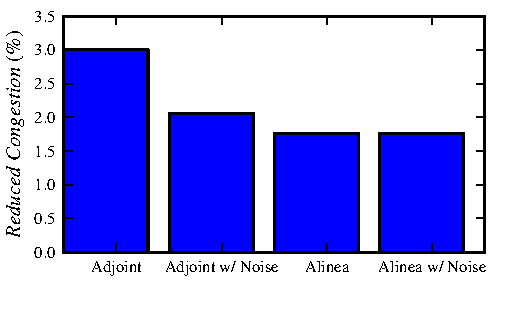
\includegraphics[width=0.45\columnwidth]{images/longmpc}
																				
										}\hfill{}\subfloat[Reduced congestion with increasing sensor noise.\label{fig:Ramp-metering-performance-1}]{\includegraphics[width=0.45\columnwidth]{images/noiseplot}
									}
									\caption{Summary of ramp metering simulations on I15 South netowrks.}
								\end{figure}
																
																
																
								\subparagraph{Robustness to noise.}
																
								Simulation results on the synthetic network with varying levels of
								noise are shown in Figure~\ref{fig:Ramp-metering-performance-1}.
								The adjoint method is able to outperform the Alinea method when the
								noise level is less than 80\%, a reasonable assumption for data provided
								by well-maintained loop detectors. As the initial and boundary condition
								data deteriorates, the adjoint method becomes useless. Since Alinea
								does not rely on boundary data, it is able to produce improvements,
								even with severely noisy data. The results indicate that the adjoint
								method will outperform Alinea under reasonable noise levels in the
								sensor data.
